\documentclass[12pt, openany]{report}
\usepackage[utf8]{inputenc}
\usepackage[T1]{fontenc}
\usepackage[a4paper,left=2cm,right=2cm,top=2cm,bottom=2cm]{geometry}
\usepackage[frenchb]{babel}
\usepackage[pdftex]{graphicx}
\usepackage{amsmath,amsfonts,amssymb}
\usepackage{hyperref}
\usepackage{color}
\usepackage[table]{xcolor}
\usepackage{listings}
\usepackage{enumitem}
\usepackage{pifont}
\usepackage{ragged2e}
\usepackage{tabto}
\usepackage{float}


\setlength{\parindent}{0cm}
\setlength{\parskip}{1ex plus 0.5ex minus 0.2ex}
\newcommand{\hsp}{\hspace{20pt}}
\newcommand{\HRule}{\rule{\linewidth}{0.5mm}}
%\renewcommand{\thesection}{\Roman{section}}
\renewcommand{\thesection}{\arabic{section}} 
\setcounter{secnumdepth}{4}
\setcounter{tocdepth}{4}

%contenu du document
\begin{document}


\begin{titlepage}
  \begin{sffamily}
  \begin{center}
	
\includegraphics[scale=0.5]{ub.png}~\\[1cm]

    \textsc{\Large MASTER 2 Informatique RCI }\\[1.5cm]
    2021-2022

    % Titre
    \rule{1\linewidth}{2pt}
     \\[1cm]
    { \huge \bfseries Rapport de PFE :\\
    Déploiement d'un VPN sur des équipements mobiles ou IoT\\[1cm] }
    \rule{1\linewidth}{2pt}
    \\[1cm]
    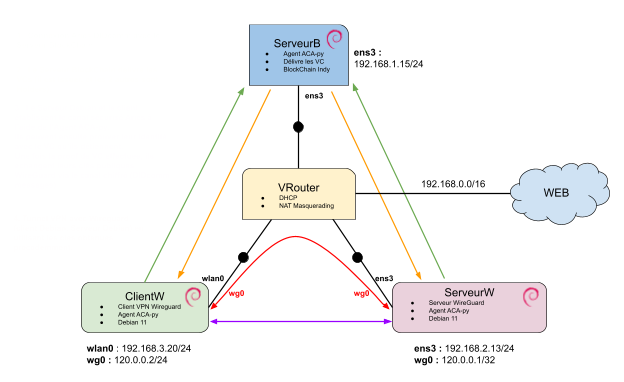
\includegraphics[scale=0.37]{topo.png}
    \\ %[1cm]

    % Membres du groupe
   \vfill
      \begin{center}
        %\hspace*{3.1cm}
        \Large	 Alexis Henquinet \hspace*{1cm} Mohamed Diallo \hspace*{1cm} Sara Real Santos
      \end{center}
 
    % Bas de la page
 
  \end{center}
  \end{sffamily}
\end{titlepage}

\newpage

\renewcommand{\contentsname}{Sommaire}
%\addcontentsline{toc}{section}{Remerciements}
\tableofcontents
\newpage

\section{Introduction}
\subsection{Contexte}
\noindent 
\begin{flushleft}
De nos jours l'emploi de réseaux privés virtuels (VPN, Virtual Private Network) est de plus en plus démocratisé. On s'en sert généralement pour masquer son adresse ip, ou pour créer un canal sécurisé chiffré avec un destinataire. De nombreuses applications, services et protocoles de VPN différents existent, que ce soit sur Ordinateur ou Smartphone.\\
En tant qu'utilisateur, se connecter à un serveur VPN nécessite d'en connaitre son adresse ip ainsi qu'échanger des clés de chiffrement (symétrique ou asymétriques) avec celui-ci. Cependant pour garantir l'authenticité de la connexion, et identifier le serveur/client avec lequel le tunnel VPN s'établit, on peut recourir aux Certificats. Lorsqu'un client veut se connecter à un serveur, il lui demande son certificat afin de prouver son identité. Ce certificat étant délivré par un tier de confiance, à savoir l'Autorité de certification, le client peut donc avoir une preuve de l'identité du serveur. Cependant, ce système étant centralisé, il dépend des autorités de certification et peut présenter différents problèmes. D'une part la possible censure ou contrôle de la part de cette autorité, mais aussi le fait que si jamais cette autorité est attaquée, alors tous les certificats délivrés par celle-ci sont compromis. Pour pouvoir contrer ces difficultés, de nouvelles méthodes basée sur la décentralisation des autorités de certifications existent, comme par exemple basées sur la BlockChain.\\
\end{flushleft}

\subsection{Présentation du projet}
\noindent 
\begin{flushleft}
\textit{Déploiement d'un VPN sur des équipement mobiles ou IoT} est un projet dont le but est de réussir à installer et configurer le VPN WireGuard sur un client Android. Cet Android sera une machine virtuelle qui s'appuie sur les logiciels QEMU et KVM, et membre d'un réseau virtuel NEmu.\\
WireGuard est un VPN nécessitant des couples de clés publique/privée de chiffrement asymétrique. Afin de garantir l'authentification et l'identité du serveur VPN WireGuard auquel le client Android se connectera, cela nécessitera l'emploi de Verifiable Credentials (VC), un équivalent des Certificats mais dont l'autorité de certification repose sur la décentralisation, à savoir un noeud de blockchain déjà existant. Le projet Aries Hyperledger soutenu par la fondation Linux permet de développer des mécanismes basés sur les VCs. Nous utiliserons donc Aries Mobile Agent sur le client Android pour communiquer avec un Aries Cloud Agent relié à un réseau Hyperledger Indy dont le rôle est de délivrer les VC. Nous utiliserons également un Aries Cloud Agent sur le serveur WireGuard afin de communiquer avec le noeud Indy et récupérer un VC.
\end{flushleft}

\newpage
\section{Étude de l'existant}

\subsection{Wireguard}
\noindent 
\begin{center}

\includegraphics[width=\textwidth]{wg.png}
\end{center}

\begin{flushleft}
WireGuard est un VPN fonctionnant sur la couche 3 du modèle OSI. Il est implémenté comme une interface réseau virtuelle du noyau pour Linux. Il est pensé pour remplacer les VPN IPsec et ceux basés sur TLS comme OpenVPN, tout en se voulant plus sûr, performant et facile d'utilisation de part son implémentation en moins de 4000 lignes de code facilement compréhensibles et vérifiables sur les systèmes Linux.\\
Il a été initialement déployé pour les systèmes Linux, mais il dispose maintenant de portages sous Android, Windows ou macOS principalement. Pour un client, WireGuard ne nécessite qu'un échange de clés publiques et d'informations de connexions comme l'adresse ip du serveur hôte. De courtes clés statiques pré-partagées en Curve25519 (basé sur Diffie-Hellman) sont utilisées pour l'authentification mutuelle. Le protocole proposé assure une confidentialité forte ainsi qu'un haut degré de dissimulation d'identité. Au niveau du transport, il utilise le cryptage authentifié ChaCha20Poly1305 pour l'encapsulation des paquets en UDP.  La clé publique construite avec Curve25519 est utilisée pour créer une interface réseau qui lui est associée. Ces interfaces font partie de la 'cryptokey routing table', qui peut être configuré et à laquelle on peut ajouter des règles de routage supplémentaires. Quand des paquets sont envoyés vers une machine par un tunnel Wireguard (donc, par l'interface dans la cryptokey routing table), ils sont chiffrés avec la clé publique de la machine qui reçoit le paquet.\\
Il est cependant à noter que les couples de clés asymétriques publiques/privées génrérées par WireGuard à l'aide de son algorithme ne sont pas adaptables aux Certificats X509 de part leur format (32 caractères 64 bits).\\
Nous utiliserons pour notre projet la version mobile Android de WireGuard côté client, ainsi que la version Linux de WireGuard côté serveur.

\end{flushleft}

\subsection{Verifiable Credentials}
\noindent 
\begin{flushleft}
Un "credential" correspond à une accréditation, un certificat ou une référence. Par exemple dans le monde physique cela peut être une pièce d'identité, un passeport, un permis ou encore un diplôme universitaire. Avec l'avènement de la BlockChain, il est maintenant possible de représenter numériquement et de manière sûre un credential. On parle alors de Verifiable Credential, car grâce à la BlockChain il est possible de les vérifier facilement et rapidement. En Novembre 2019 le W3C a entammé une procédure de normalisation en publiant une recommandation sur les Verifiable Credentials, dans le but de garantir un format générique reconnu mondialement. Il s'agit donc d'une technologie novatrice et en pleine construction.\\
Il y est stipulé qu'un détenteur (ou "Holder") de VC peut générer une présentation à partager à quelqu'un voulant une preuve d'accréditation selon certaines caractéristiques, et ce sans forcément transmettre l'entièreté des caractéristiques de son VC. Par exemple pour obtenir un service nécessitant d'être majeur, une preuve de notre âge peut nous être demandée. Il n'est alors pas obligatoire de transmettre le champ de son VC d'identité contenant sa date de naissance, mais par exemple juste prouver dans la présentation que l'on a "plus de 18 ans".\\

Pour mieux comprendre les différents rôles et informations concernant les VCs, voici ci-dessous le schéma proposé par la W3C :\\
\begin{figure}[h]
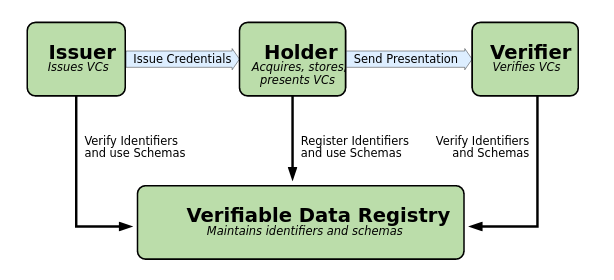
\includegraphics[scale=0.5]{vc.png}
\centering
\caption{Schema des rôles et des échanges d'information}
\end{figure}

Des mécanismes de preuves et de signatures numériques sont nécessaires afin d'assurer la protection d'un Verifiable Credential. L'obtention de la validation des preuves peut dépendre de la syntaxe de la preuve, cependant dans le cadre de ce projet les VCs correspondront à des JSON Web Tokens sécurisés par l'utilisation de JSON Web Signatures. Voici ci-dessous un exemple de de VC JWT présenté par le W3C :\\
\begin{figure}[h]
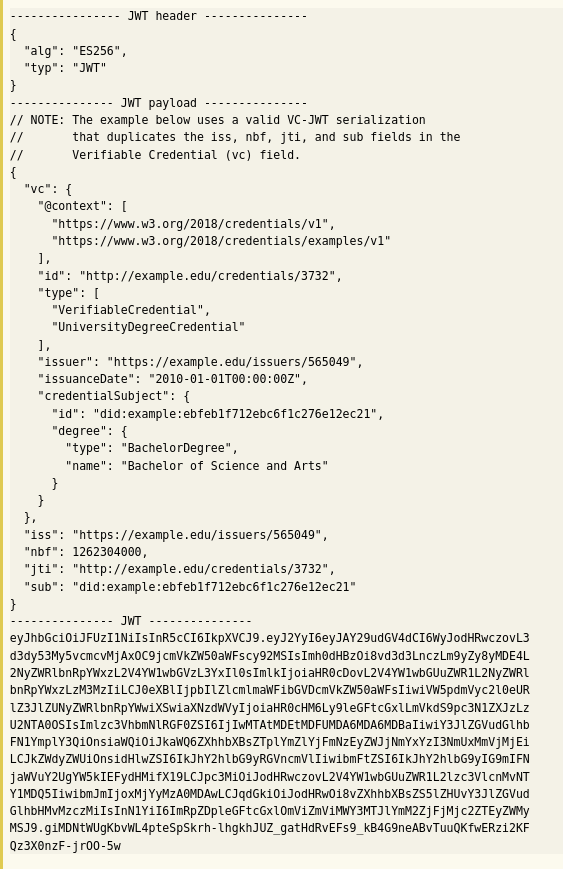
\includegraphics[scale=0.4]{vc2.png}
\centering
\end{figure}

\end{flushleft}

\newpage
\subsection{Aries Hyperledger}
\noindent 
\begin{flushleft}
Aries Hyperledger est un projet developpé par l'Hyperledger Foundation. Hyperledger Foundation est une communauté centrée sur le développement d'outils, librairies et frameworks permettant de déployer des blockchains qui seront majoritairement utilisées par des entreprises. \\
Il y a différents projets lancées par la Fondation Hyperledger. Aries Hyperledger est le 13ème projet fondé par cette communauté. Aries Hyperledger est une infrastructure permettant l'échange de données en relation à une blockchain ainsi que l'échange de messages en peer-to-peer. \\
\vspace{2mm}
Aries Hyperledger inclut plusieurs services dans son infrastructure :
\begin{itemize}
\item Une couche interface appelée \textbf{resolver} qui permet de créer et signer des transactions blockchain.
\item Un \textbf{wallet} sécurisé permettant de garder des secrets et autres informations. 
\item Un système de \textbf{messagerie} encryptée pour l'échange entre clients hors blockchain.
\item Une implémentation des \textbf{W3C Verifiable Credentials} 
\item Une implémentation du Decentralized Key Management System (DKMS).
\item Un méchanisme qui permet de construire des protocoles et des API.

\end{itemize}
\begin{figure}[h]
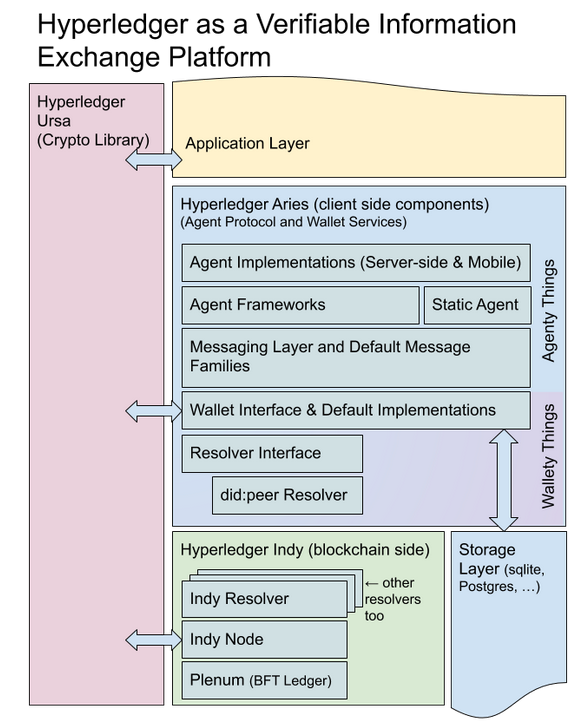
\includegraphics[scale=0.4]{aries-hyper.png}
\centering
\caption{Différents projets Aries et leur intéractions}
\end{figure}

\vspace{5mm}
Le plus grand objectif du projet Aries Hyperledger est de pouvoir offrir une infrastructure capable de s'adapter et de travailler avec des technologies développées par Indy ou qui se servent d'autres technologies blockchain. 
\end{flushleft}

\newpage
\subsubsection{Aries Cloud Agent}
\noindent 
\begin{flushleft}
Hyperledger Aries Cloud Agent Python (ACA-Py) est une projet visant à servir de base pour contruire des Agents pouvant utiliser des Verifiable Credentials. Ses protocols et fonctionnalités de base permettent de délivrer, vérifier et stocker des Verifiable Credentials. Les agent ACA-Py peuvent contrôler des Verifiable Credentials de format Hyperledger Indy AnonCreds et de format W3C. Dans ce projet nous nous intéréssons au dernier format proposé, le W3C. \\
Aries Cloud Agent fonctionne avec des requêtes HTTP et des notifications webhook. Ceci donne la possibilité aux développeurs d'écrire un controlleur qui 'discute' avec notre agent en n'importe quel langage pouvant gérer des requêtes HTTP. \\
L'Agent Aries Cloud met aussi en oeuvre une interface OpenAPI REST pouvant servir à comprendre comment les protocols dans notre agent fonctionnent. Le dévéloppeur peut donc utiliser ceci pour gérer le comportement de l'agent. Voici un résumé de l'architecture de l'agent Aries Cloud : \\

\begin{figure}[h]
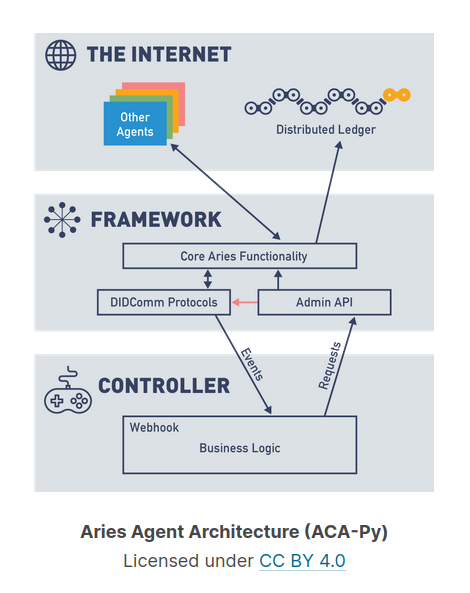
\includegraphics[scale=0.5]{ACA-py.png}
\centering
\caption{Architecture d'un Agent Aries}
\end{figure}
\end{flushleft}

\vspace{2mm}
Dans l'architecture ci-dessus, nous pouvons voir que l' Agent communique avec un Distributed Ledger, donc un Blockchain. Pour précision, dans notre projet nous utilisons Von Network comme réseau Blockchain.

\vspace{2mm}
Pour contrôler et agir dans l'API il suffit juste de retrouver l'endpoint qui se charge de la requête que nous voulons exécuter, le sélectionner et rentrer les champs nécessaires s'il en faut. C'est un outil très efficace pour comprendre et développer son propre agent. On peut en voir un exemple ci-dessous :\\
\begin{figure}[H]
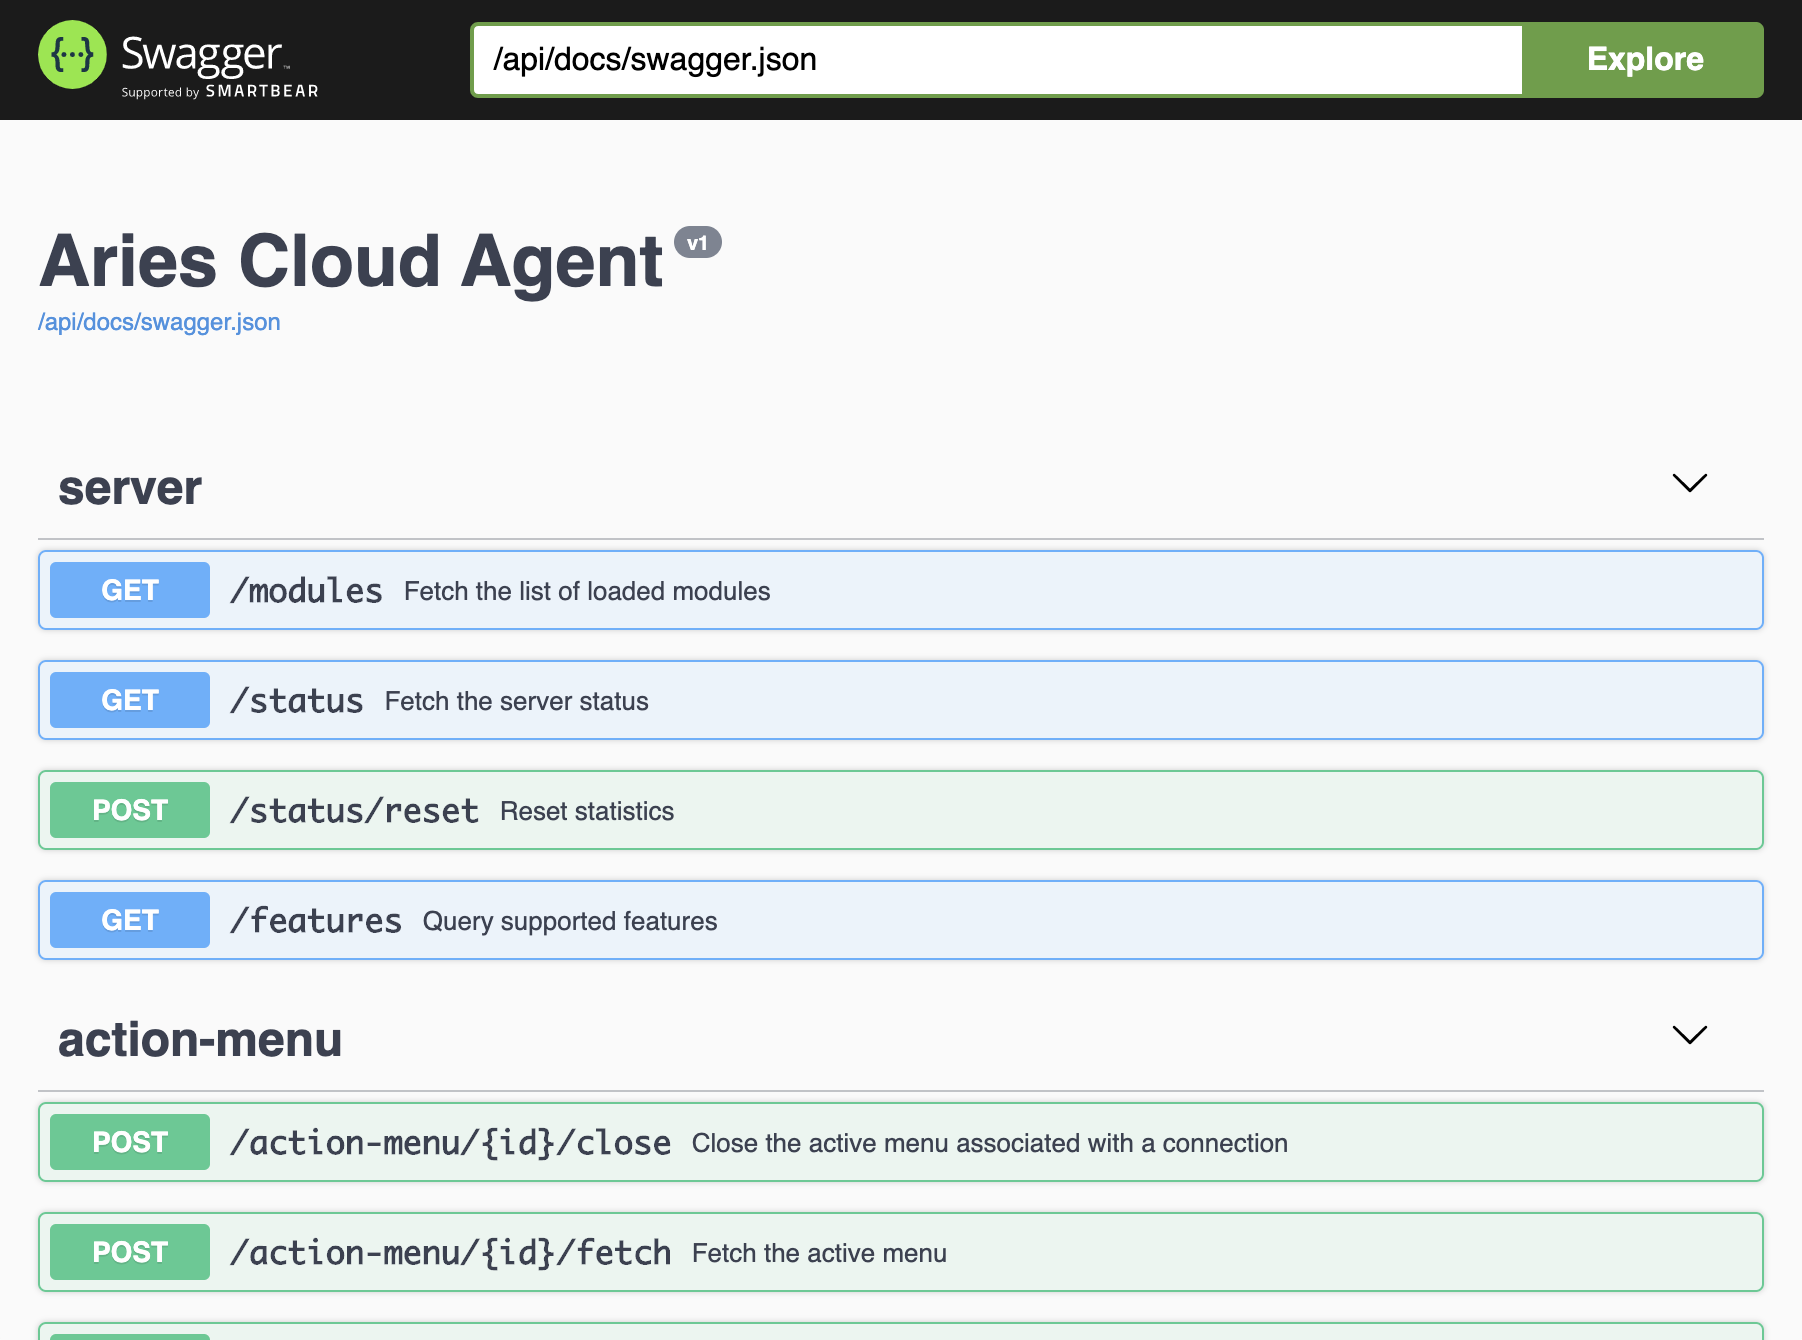
\includegraphics[scale=0.17]{adminApi.png}
\centering
\caption{API d'un Aries Cloud Agent}
\end{figure}


\subsubsection{Aries Mobile Agent React-Native}
\noindent 
\begin{flushleft}
L'Aries Mobile Agent (ou Aries Bifold) est une application Open Source développée sur React Native 0.64.1 qui a pour but de regrouper les efforts de la communauté Aries Hyperledger orientée application mobile vers un projet centralisé, afin d'éviter la duplication du code et les similitudes entre les projets. Ce projet est aussi destiné à aider d'autres projets spécifiques voulant utiliser sur mobile les technologies de la fondation Aries Hyperledger sans avoir à redéfinir la complexité interne des agents Aries. Il est conçu pour permettre de démarrer rapidement un projet en ayant un agent Aries de base.\

Aries Mobile Agent est basé sur deux dépendances principales qui sont les suivantes :\\
\begin{itemize}

\item Aries Framework Javascript, un framework écrit en TypeScript pour la création d'agents Self Sovereign Identity. SSI est une approche visant l'idée que chacun contrôle ses propres données informatiques, ainsi qu'un contrôle de quand et comment elles sont fournies aux autres. De plus, lorsqu'une donnée est partagée, cela doit être fait avec fiabilité. Avec SSI, il n'y a pas d'autorité centrale détenant les données les transmettant à d'autres entités sur demande. Vous seul en êtes le possesseur. Ce framework a également pour but d'utiliser les services DIDComm qui visent à être en conformité avec les normes définies dans les RFC d'Aries.

\item Indy-sdk-react-Native : Il s’agit d’un Wrapper de Indy destiné à React Native. Son rôle est d’implémenter les fonctionnalités de Indy SDK afin qu’elles soient utilisables avec React Native. 

React Native est un framework d'applications mobiles Open Source conçu par Facebook. Il est utilisé pour développer des applications natives pour Android et iOS. Aries Bifold étant développé en React native 0.64.1, il cible l’API 29.0.3 d’Android, tandis que sur IOS il vise la version 10.0+ et il ne peut être utilisé que sur des appareils physiques pour le moment. La virtualisation est possible que sur Androidx86.

Aries Bifold nécessite un médiateur pour fonctionner. Le mobile Agent est configuré pour utiliser la médiation implicite. Il utilise par défaut Indicio Public Mediator, médiateur public de tests en ligne basé sur un Agent ACA-Py.
Un médiateur est un agent dont le but est de faire l'intermédiaire entre un Mobile Agent et un autre Agent (par exemple un Cloud Agent ACA-py), en relayant les messages transmis entre eux. Une connexion DIDComm est établie avec le médiateur.\
Ci-dessous nous pouvons voir le principe et fonctionnement d'un médiateur entre deux Agents Alice et Bob comme cela est présenté dans la norme "Aries RFC 0211: Coordinate Mediation Protocol"\footnote{\url{https://github.com/hyperledger/aries-rfcs/blob/main/features/0211-route-coordination/README.md
}} :\\

\begin{center}
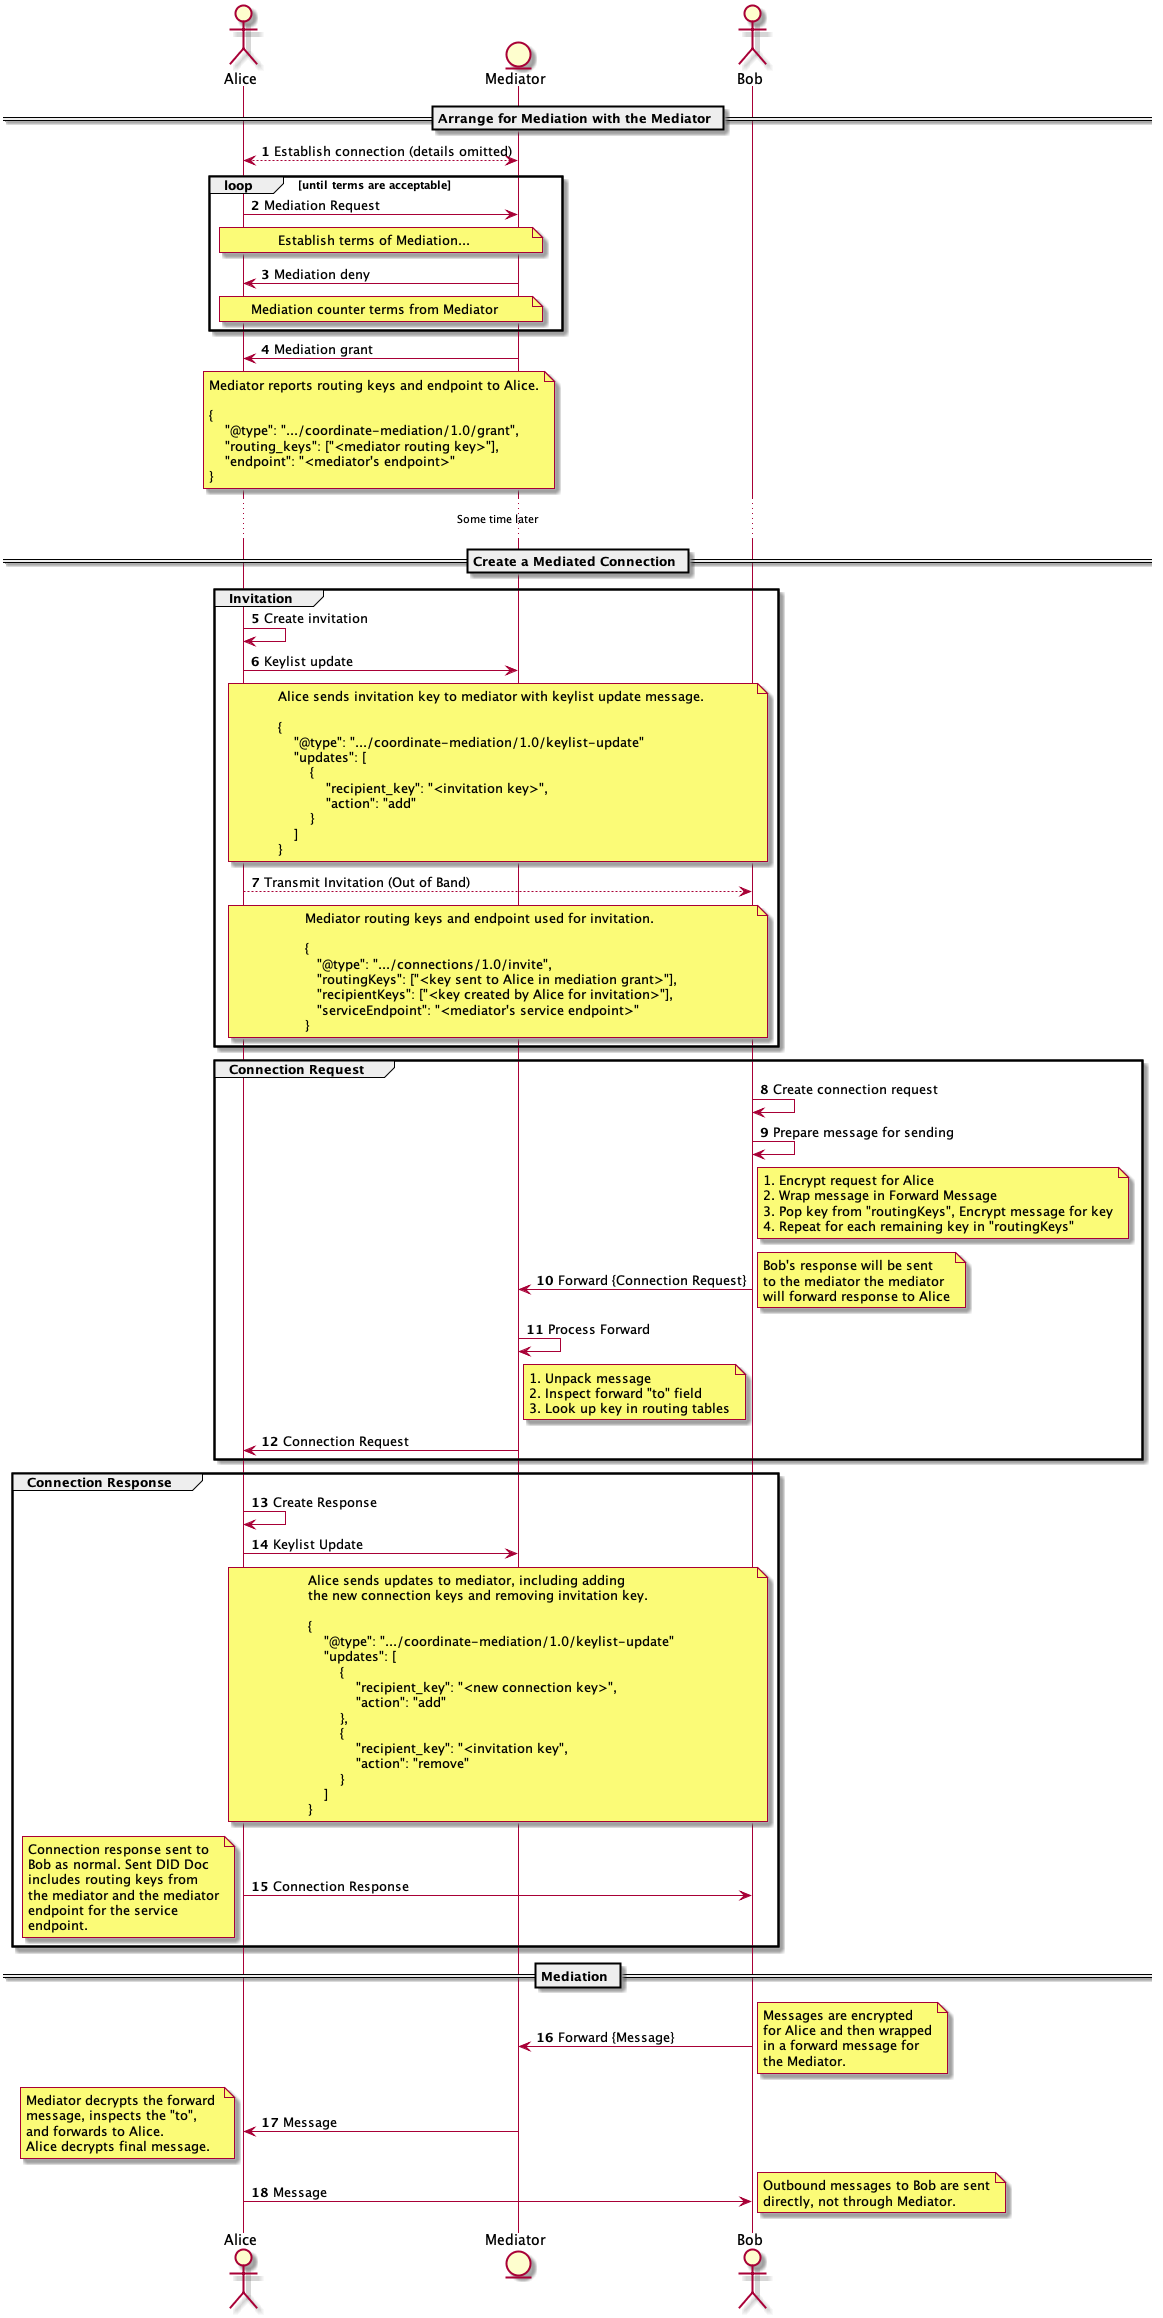
\includegraphics[scale=0.25]{mediator.png}
\end{center}

\end{itemize} 
\end{flushleft}

\subsection{QEMU}
\noindent 
\begin{center}

\includegraphics[scale=0.2]{qemu.png}
\end{center}
\begin{flushleft}
QEMU est un logiciel libre  pouvant émuler un processeur ou une architecture différente. Il peut émuler un système ou juste le virtualiser, dépendant du système de l'hôte. QEMU peut exécuter différents systèmes d'exploitation et leurs applications de manière isolée sur une même machine physique ainsi que simuler les périphériques. \\
Dans notre projet nous nous sommes servis de QEMU pour émuler deux machines Debian11 et une machine Androidx86. Cependant, pour des raisons techniques expliquées plus tard, nous avons dû remplacer la machine Androidx86 par une autre machine Debian11. 
\end{flushleft}

\subsection{NEmu}
\noindent 
\begin{flushleft}
NEmu pour Network Emulator for Mobile Universes est un environnement permettant de mettre en place des réseaux virtuels développé par Monsieur Vincent Autefage. NEmu permet de construire un environnement virtuel distribué ne nécessitant pas de droits d'administration pour fonctionner. Il contrôle un ensemble de machines virtuelles QEMU dans le but de construire une topologie de réseau virtuel. Il dispose d'une API python rendant le travail plus facile. Il dispose également de fonctionnalités de simulation de dispositifs réseaux comme des routeurs, des switchs ou encore des Smartphones pour étendre ses fonctionnalités et administrer avec plus de facilité un réseau. \\
Dans le cadre de ce projet nous devons utiliser NEmu pour construire le réseau virtuel sur lequel nous simulerons les interactions entre Agents Aries et le VPN WireGuard.
\end{flushleft}

\section{Scénarios}
L'objectif de ce projet était d'installer et configurer un VPN Wireguard tout en utilisant la technologie Blockchain à la place de certificats pour s'authentifier et échanger des clés publiques. 

\subsection{Scénario initial}
\noindent 
\begin{flushleft}
Le premier scénario de ce projet était composé de deux machines Debian11 et d'une machine Androidx86. Ces trois machines appartennaient toutes au même réseau. Afin de fournir à la fois un accès à internet et au réseau local, un routeur virtuel délivrant les services dnsmsak, dhcp et Masquerading reliait les 3 machines à internet et leur fournissait leurs adresses ip.\\
\vspace{2mm}
Il y avait 3 types d'Agent à mettre en place : un Cloud Agent pour la machine Serveur Blockchain, un Cloud Agent pour la machine Serveur Wireguard et un Static Agent pour la machine Android. \\
Le Serveur Blockchain devait générer des clés publiques compatibles avec WireGuard en utilisant OpenSSL, les mettre dans un Verifiable Credential et les envoyer au Client et au Serveur Wireguard. \\
Cependant, après des recherches nous avons constaté que ce scénario avait des problèmes limitant son implémentation. Le principal problème concernait le Static Agent. Le Static Agent était sensé être implémenté sur le Client Android, mais nous avons découvert après s'être penchés en détail sur sa documentation ainsi qu'effectué des tests qu'il n'avait pas de wallet. Il ne peut donc pas stocker des Verifiable Credentials. Cet Agent a été pensé seulement pour établir une communication DIDComm avec un CloudAgent, et échanger en peer-to-peer de simples messages DIDComm.
\end{flushleft}

\subsection{Scénario intermédiaire}
\noindent
\begin{flushleft}
Après avoir testé et démontré que le Static Agent n'était pas utilisable dans le cadre de ce projet, nous avons du modifier notre scénario initial. Le Static Agent sur le client Mobile Android a été remplacé par un projet novateur cherchant à implémenter un équivalent de Cloud Agent sur Mobile, à savoir le projet Aries Mobile Agent React Native.\\
Notre scénario intermédiaire était donc composé de deux machines Debian11 implémentant toutes les deux des Cloud Agents, et une machine Androidx86 implémentant un Mobile Agent. \\
\vspace{2mm}
Malheureusement lors des tests et de l'implémentation du Mobile Agent dans le but de l'adapter à notre projet, nous nous sommes heurtés à de nombreux problèmes. Le projet Aries Mobile Agent est un projet réçent toujours en cours de développement dont le but est de centraliser toutes les avancées dans les portage sous mobile d'Agents Aries Hyperledgers. Comme nous le détaillerons plus tard dans la partie lui étant concernée, nous nous sommes heurtés à des problèmes de compatibilité entre ce Mobile Agent et les Cloud Agents de nos machines. Nous avons donc décidé de remplacer ce Mobile Agent sur le Client Wireguard par un Cloud Agent classique. Comme le Cloud Agent n'est pas prévu pour fonctionner sur Android, nous avons utilisé Debian11 à la place. \\
\vspace{2mm}
Au niveau des clés Wireguard, OpenSSL n'est pas capable de générer des clés Wireguard. En effet, WireGuard utilise un Algorithme propriétaire pour générer des paires de clés X25519 qui sont une méthode d'accord de clé et donc pas utilisables pour la signature. Donc chaque machine Wireguard devra générer ses propres clés en utilisant l'algorithme de Wireguard.
\end{flushleft}

\subsection{Scénario fonctionnel}
\noindent
\begin{flushleft}
Notre scénario final est composé de trois machines Debian11. Les trois implémentent un Cloud Agent. Chaque machine appartient à un sous-réseau différent du VRouter possédant les services dnsmask, dhcp et NAT Masquerading. Le routeur garantit l'accessibilité entre les différentes machines virtuelles ServeurB, ServeurW et ClientW.\\
Les clés Wireguard sont générées en utilisant l'algorithme de Wireguard par le ClientW et le ServeurW Wireguard, puis envoyées au Serveur Blockchain qui les stocke dans des Verifiable Credential. Ces Verifiable Credentials sont envoyés aux machines Wireguard et utilisés pour s'authentifier et s'échanger les clés afin de mettre en place un tunnel VPN Wireguard. Dans ce scénario, il a été convenu que les deux machines WireGuard doivent s'authentifier mutuellement.
\end{flushleft}

\section{Architecture et implémentation}

\subsection{Réseau virtuel NEmu}
\noindent 
\begin{flushleft}

Nous avons mis en place un réseau virtuel à l'aide de NEmu pour mettre en relation notre Serveur Blockchain ServeurB, notre Serveur Wireguard ServeurW et notre Client Wireguard ClientW. Chaque machine se trouve dans un sous-réseau différent : 
\begin{itemize}
\item \textbf{Serveur Blockchain} possède l'addresse IP : 192.168.1.15/24
\item \textbf{Serveur Wireguard} possède l'addresse IP : 192.168.2.13/24
\item \textbf{Client Wireguard} possède l'adresse IP : 192.168.3.20/24
\end{itemize}
Il faut prendre en compte aussi que notre VPN Wireguard met en place une interface réseau virtuelle entre le client et le serveur, leur adresses virtuelles sont 120.0.0.2 et 120.0.0.1 respectivement. \\
Afin de faciliter la configuration des adresses et l'accès à internet, nous avons décidé d'utiliser un VRouter de NEmu. Un VRouter est un router Linux TinyCore virtuel qui simplifie la gestion des réseaux virtuels à l'aide de ses services dnsmask, dhcp et nat masquerading.

\begin{figure}[H]
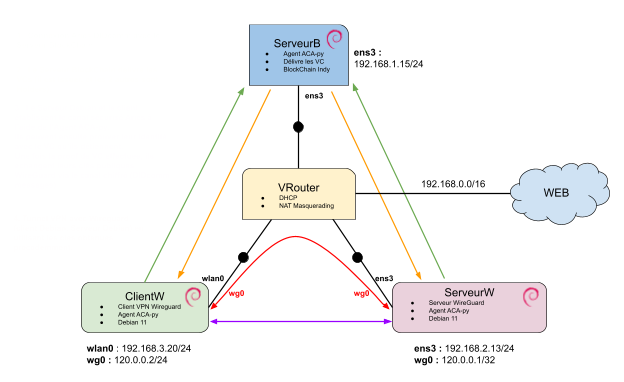
\includegraphics[scale=0.4]{topo.png}
\centering
\caption{Topologie du réseau NEmu}
\end{figure}

Le script de configuration du réseau virtuel network.py a été défini pour être utilisable au CREMI en se basant sur une seule image debian11.img (et android.img à l'origine) de base pour toutes les VMs dans /net/stockage/PFE-VPN-2022/. Cela nous as permis d'éviter d'avoir à nous transférer à chaque fois en local sur nos machines la nouvelle image de base. Par défaut le script est configuré avec un VHostConf attribuant 2 coeurs de CPU à chaque VM, ce qui suffit largement pour notre projet.\\
Afin de générer les images de base debian11.img et android.img nous avons réalisé un script creator.py.

\subsection{Choix de l'implémentation}

Au niveau des technologies utilisées pour chaque machine nous retrouvons :\\
\begin{itemize}
\item \textbf{ServeurB :} Un von-network dockerisé permettant d'obtenir un noeud de blockchain Indy + Un Aries Cloud Agent Python.
\item \textbf{ServeurW :} Un Aries Cloud Agent Python + un Serveur WireGuard.
\item \textbf{ClientW :} Un Aries cloud Agent Python + un Client WireGuard.
\end{itemize}
Le fonctionnement de notre implémentation est le suivant : 

\begin{itemize}
\color{green}
\item[1.] \color{black} Nos Agents Client et Serveur Wireguard se connectent avec le Serveur Blockchain par Aries DIDComm

\color{orange}
\item[2.] \color{black} Le Serveur BlockChain qui est considéré le \textbf{Issuer} délivre les Verifiable Credentials au Client et Serveur Wireguard qui dans ce cas sont les \textbf{Holders}.

\color{violet}
\item[3.] \color{black} Le Serveur Wireguard et le Client établissent le canal sécurisé Aries à l’aide de l’Agent ACA-py.\\
Ils peuvent ensuite prouver leur identité avec le VC qu’ils détiennent.
Une fois la proof de VC effectuée, ils échangent leurs clés publiques WireGuard via le canal chiffré (DIDcomm messages).

\color{red}
\item[4.] \color{black} Établissement du tunnel VPN avec Wireguard entre le Client et le Serveur Wireguard en utilisant les clés obtenues précédemment.

\end{itemize}


\end{flushleft}

\subsection{Cloud Agent du Serveur BlockChain}
\noindent 
\begin{flushleft}
Le serveur Blockchain est le serveur qu'est directement relié au réseau de noeuds Blockchain.  Dans le cas où on veut avoir notre propre réseau de noeuds Blockchain, le serveur Blockchain sera celui qui déploie ce réseau en utilisant Von Network pour déployer les noeuds Blockchain. Nous avons aussi la possibilité de prendre comme référence un réseau de noeuds déjà éxistant. \\

\begin{figure}[h]
\vspace{2mm}
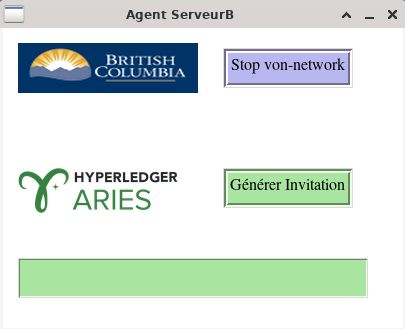
\includegraphics[scale=0.7]{serveurB.png}
\centering
\caption{Interface graphique de notre Serveur Blockchain}
\end{figure}

Le Serveur Blockvhain est l'acteur qu'enregistre les utilisateur auprès de la Blockchain. Il enregistre aussi les schemas et les définitions de credentials. Les Schemas et Définitions de Credentials permettent de mettre en place un format et des champs pour les Verifiable Credentials. Les Verifiable Credentials que nous avons choisi d'utiliser ont deux champs : un champ pour la \textbf{clé publique} et un autre pour le nom de la machine qui détient ce Verifiable Credential. Il y a aussi un champ contenant la signature du Verifiable Credential.\\

\begin{figure}[H]
	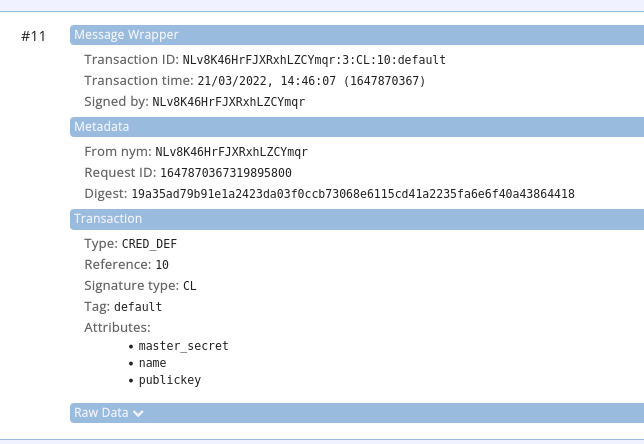
\includegraphics[scale=0.5]{cred_def.png}
	\centering
	\caption{Définition de notre Credential}
\end{figure}

\end{flushleft}



\subsection{Cloud Agent du Serveur WireGuard}
\noindent 
\begin{flushleft}
Le Serveur Wireguard est une machine Debian qui hoste un service VPN Wireguard.  Dans cette machine il y a aussi un Agent Cloud. Cet Agent Cloud est capable de communiquer avec d'autres agents, notamment dans ce cas l'Agent du Serveur Blockchain et l'Agent du Client Wireguard. Il aura de différentes intéractions avec chacun des deux agents. \\
\vspace{2mm}
Avec l'Agent Server Blockchain il aura des interactions ayant comme objectif la réception de Verifiable Credentials. Le Serveur Wireguard génère des clés Wireguard et envoie sa clé publique dans une proposal de Verifiable Credential. Un proposal est une proposition de VC basée sur une Definition de Credential ( celle que nous avons enregistrée avec le Serveur Blockchain ). Le Serveur Blockchain lui délivre un VC avec la clé publique et son nom. \\
\vspace{2mm}
Les échanges avec le Client Wireguard seront différents. En premier, le Serveur Wireguard doit répondre aux requêtes de preuves de la part du Client Wireguard. Le Serveur Wireguard doit en premier lieu produire une Verifiable Presentation puis l'envoyer. Cette Verifiable Presentation dépend de la requête du Client Wireguard, c'est à dire, la construction et les champs inclus dans cette Presentation dépendent de ce que le Client demande. Normalement, il va envoyer une Verifiable Presentation contenant sa clé publique et son 'nom'. \\
Dans la requête de preuve, le Client inclut sa clé publique Wireguard. Une fois que notre présentation est bien validée, le client aura récuperé notre clé publique. Finalement, le VPN Wireguard peut être mis en place des deux côtés. \\

Nous avons mis en place une interface graphique en python pour pouvoir gérer les différentes intéractions et événements.\\

\begin{figure}[H]
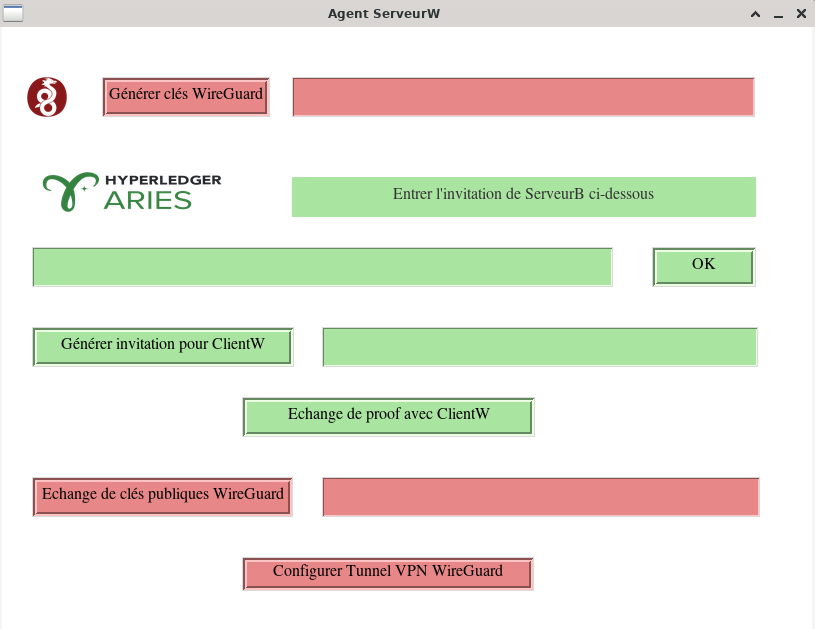
\includegraphics[scale=0.5]{serveurW.png}
\centering
\caption{Interface graphique de notre Serveur Wireguard}
\end{figure}

\end{flushleft}

\subsection{Agent du Client WireGuard}
\subsubsection{Mobile Agent}
\noindent
\begin{flushleft}

\end{flushleft}


\subsubsection{Cloud Agent}
\noindent 
\begin{flushleft}
Le Client Wireguard est une machine Debian qui a comme finalité se connecter sur le VPN du serveur Wireguard. \\
Comme pour le Serveur Wireguard, le Serveur Blockchain doit délivrer un Verifiable Credential avec la clé publique Wireguard du client dedans. Ceci se fait avec une proposal de Verifiable Credential. \\
Quand le Client voudra se connecter sur le Serveur Wireguard, il devra en premier faire une requête de preuve auprès du Serveur Wireguard, contenant la clé publique du client et demandant entre autres, la clé publique du serveur. Celui-ci envoie une Verifiable Presentation avec sa clé publique Wireguard. La requête du client contennait aussi sa clé publique, donc quand la Presentation est validé, le serveur et client Wireguard ont tous les deux les clés de l'autre.

\end{flushleft}




\section{Analyse du fonctionnement \& Tests}
\noindent 
\begin{flushleft}

\subsection{Analyse du fonctionnement}
Tous les modules de notre application fonctionnent, les tests permettent d'assurer que les bugs ou erreurs majeurs n'apparaissent pas pendant l'utilisation de l'application.\\
Bien entendu que, une partie de notre code à savoir le ServeurB, ClientW, ServeurW excecute des commandes \textbf{Aries Cloud Agent - Python} et \textbf{von-network} (qui sont en cours de développement, soit importés ailleurs), augmentent considérablement les différents cas d'erreurs et tous n'ont pas pus être testés.  
\subsection{Tests}

\subsubsection{Test de couverture}

\begin{figure}[H]
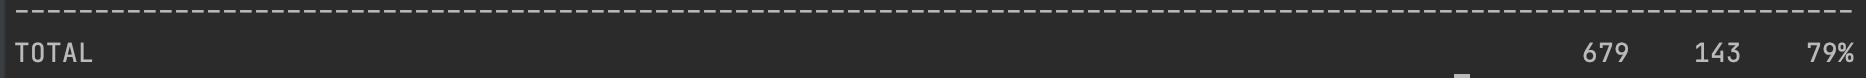
\includegraphics[scale=0.5]{coverage.png}
\centering
\caption{Resultat des tests de couverture}
\end{figure}

\subsubsection{Discussion des résultats}
Quand on observe les pourcentages obtenus par rapport aux différents codes que nous avons produit, on note que le ServerB est le moins couvert. Parce que les tests du serverB sont plus complexe à faire et il ne nous reste pas beaucoup de temps.

\end{flushleft}


\section{Conclusion}
\noindent 
\begin{flushleft}
TODO
\end{flushleft}
\subsection{Limitations}
\noindent 
\begin{flushleft}
TODO
\end{flushleft}
\subsection{Extensions}
\noindent 
\begin{flushleft}
TODO
\end{flushleft}

\section{Bibliographie}
\noindent 
\begin{itemize}

\item WireGuard : \url{https://www.wireguard.com/} (consulté le 06/03/2022) 
\item World Wide Web Consortium (W3C) : \url{https://www.w3.org/} (consulté le 06/03/2022)
\item Verifiable Credentials : \url{https://www.w3.org/TR/vc-data-model/} (consulté le 06/03/2022) 
\item Aries Cloud Agent : \url{https://github.com/hyperledger/aries-cloudagent-python} (consulté le 15/03/2022)
\item QEMU : \url{https://www.qemu.org/} , \url{https://wiki.qemu.org/Main_Page} (consulté le 15/03/2022)
\item NEmu : \url{https://gitlab.com/v-a/nemu} (consulté le 15/03/2022)

\end{itemize}

\section{Annexe}
\noindent 
\begin{flushleft}
TODO
\end{flushleft}

\end{document}

%\begin{thebibliography}{}
%\bibitem[1]{1}
%https://www.wireguard.com/

%\end{thebibliography}
